\chapter{Costruzione di un automa caratteristico LR(0) o LR(1)}
(data un'appropriata istanziazione di $P_0$ (stato iniziale) e closure function)

Prima di tutto facciamo la costruzione dell'automa caratteristico, usando l'algoritmo sotto riportato.

Istanziando $P_0$, closure otteniamo:
\begin{itemize}
	\item automi caratteristici LR(0)-automi $\leftarrow$ parsing SLR(1)\\
	\item automi caratteristici LR(1)-automi $\leftarrow$ parsing LR(1)\\
\end{itemize}
Lookahead function $LA:(FxP) \rightarrow p(T \cup \{ \$ \} )$
con F = insieme degli stati finali dell'automa caratteristico considerato. Si considerano stati finali gli stati che contengono almeno un reducing item.

L'automa caratteristico sar\'a necessario per la creazione della tabella di parsing.

\begin{lstlisting}
	Inizializzare la collezione Q di stati come {P_0};
	flag P_0 come non-marcato;

	while(ho uno stato non marcato P in Q){
		marca P;
		foreach(A -> a.Ybeta in P){
			tmp.add( A->aY.beta );
		}
		if(tmp == kernel(R)){ //per qualche R in Q
			tau(P, Y) = R;
		} else {
			newState = closure(tmp);
			tau(P, Y) = newState;
			Q.add(newState); //come non-marcato 
		}
	}
\end{lstlisting}

Forse come eseguire la chiusura:
se ho la grammatica:
$S' \rightarrow S$\\
$S \rightarrow aSb|ab$\\
$closure_0(\{ S' \rightarrow .S\})$ \'e composta da:\\
$S \rightarrow .aSb$\\
$S \rightarrow .ab$\\

Se invece ho una grammatica tipo 
$E' \rightarrow E$\\
$E \rightarrow E + T | T$\\
$T \rightarrow T * F | F$\\
$F \rightarrow (E) | id $\\

Allora $closure_0(\{ E' \rightarrow .E \})$ diventa
$E \rightarrow .E + T $ quelle con il punto prima della E le ho gi\'a aggiunte, non faccio nulla\\
$E \rightarrow .T $ ora aggiungo quelle con il punto prima della T\\
$T \rightarrow .T * F $ quelle con il punto prima della T le ho gi\'a aggiunte, non faccio nulla\\
$T \rightarrow .F $ ora aggiungo quelle con il punto prima della F\\
$F \rightarrow .(E)$ terminale dopo il punto, non devo aggiungere nulla\\
$F \rightarrow .id$ terminale dopo il punto, non devo aggiungere nulla\\
Si devono fare in ordine per non dimenticarsene in giro.

%%%%%%%%%%%%%%%%%%%%%%%%%%%%%%%%%%%%%%%%%%%%%%%%%%%%%%%%%%%%%%%%%%%%%%%%%%%%%%%%%%%%%%%%%%%%%%%%%%%%%%%%%%%%%%%%%%%%%%%%%%%%%%%%%%%%
\section{Algoritmo di $closure_0(P)$}
\begin{lstlisting}
	tag ogni item in P come non-marcato

	while(ho ancora un item I non marcato in P){
		marca I;
		if(I ha la forma A -> alpha .B beta){
			foreach ((B -> Y) in P){
				if(B -> Y not in P){
					add(B -> .Ya);
					segna P come non-marcato;
				}
			}
		}
	}
	return P;
\end{lstlisting}

LR(0) automa si ricava utilizzando, nell'algoritmo di costruzione dell'automa caratteristico:
\begin{itemize}
	\item $P_0 = closure_0 ( \{ S' \rightarrow .S \} )$ per la grammatica G arricchita con $S' \rightarrow S$\\
	\item $ closure_0 $ per closure\\
\end{itemize}

%%%%%%%%%%%%%%%%%%%%%%%%%%%%%%%%%%%%%%%%%%%%%%%%%%%%%%%%%%%%%%%%%%%%%%%%%%%%%%%%%%%%%%%%%%%%%%%%%%%%%%%%%%%%%%%%%%%%%%%%%%%%%%%%%%%%
\subsection{Esempio}
$ S' \rightarrow S $\\
$ S \rightarrow aSb | ab $\\

\begin{tabular}{lll}
	$P_0=$ 	&	$S' \rightarrow .S$ 	& \\
			&	$S \rightarrow .aSb$ 	& \\
		 	&	$S \rightarrow .ab$ 	& \\
	$P_1=$ 	&	$S' \rightarrow S.$ 	& ci si arriva con una S-transizione\\
	$P_2=$ 	&	$S \rightarrow a.Sb$ 	& ci si arriva con una a-transizione\\
			&	$S \rightarrow a.b$ 	& \\
		 	&	$S \rightarrow .aSb$ 	& \\
		 	&	$S \rightarrow .ab$ 	& \\
		 	& 	$P_1$ \'e finito, guardo $P_2$ & \\
	$P_3=$ 	&	$S \rightarrow aS.b$ 	& ci si arriva con una S-transizione da $P_2$\\
	$P_4=$ 	&	$S \rightarrow ab.$ 	& ci si arriva con una b-transizione da $P_2$\\
	$P_5=$ 	&	$S \rightarrow .aSb$ 	& ci si arriva con una a-transizione da $P_2$ (stesse righe di $P_2$)\\
		 	&	$S \rightarrow .ab$ 	& la freccia quindi va da $P_2$ a $P_2$, perch\'e $P_5 \subset P_2$\\
		 	&	ora guardo $P_3$	& \\
	$P_6=$ 	&	$S \rightarrow aSb.$ 	& ci si arriva con una b-transizione da $P_3$\\
\end{tabular}  

%%%%%%%%%%%%%%%%%%%%%%%%%%%%%%%%%%%%%%%%%%%%%%%%%%%%%%%%%%%%%%%%%%%%%%%%%%%%%%%%%%%%%%%%%%%%%%%%%%%%%%%%%%%%%%%%%%%%%%%%%%%%%%%%%%%%
\section{Creazione della tabella di parsing}
Sia $\tau$ la funzione di transizione dell'automa caratteristico considerato.\\
Sia LA la lookahead function considerata.\\
La tabella di parsing bottom-up per la coppia prescelta di automa e lookahead function \'e una matrice $Q \otimes (V \cup \{ \$ \})$ 
dove Q \'e l'insieme degli stati dell'automa prescelto.

Ciascuna entry (P,Y) \'e compilata come segue:
\begin{tabular}{ll}
	inserire shift    						&	se $Y \in T \land \tau(P,Y) = R $\\
	inserire reduce $A \rightarrow \beta$   &	se $A \rightarrow \beta . \in P \land Y \in LA(P, A \rightarrow \beta) $\\
	inserire accept 						&	se $Y = \$ \land S' \rightarrow S. \in P $\\
	inserire error()						&	se $Y \in T \cup \{\$\} \land$ non \'e ancora stato inserito nulla\\
	applicando i passi precedenti 			& \\
	inserire goto R  						&	se $Y \in V\backslach T \land \tau(P,Y) = R $\\
\end{tabular}

%%%%%%%%%%%%%%%%%%%%%%%%%%%%%%%%%%%%%%%%%%%%%%%%%%%%%%%%%%%%%%%%%%%%%%%%%%%%%%%%%%%%%%%%%%%%%%%%%%%%%%%%%%%%%%%%%%%%%%%%%%%%%%%%%%%%
\subsection{Esercizio}
$SLR(1)$\\
$LR(0)$ automa \\
$LA(P, A \rightarrow \beta) = follow(A)\ \forall\ P \in Q$ (automa)\\

|numero nodo| parte che pu\'o avere conflitti | goto part|\\

\begin{tabular}{|c|c|c|c|c|}
	\hline
		& 	a 	&	b 	& 	$\$$ 	&	S 	\\
	\hline
	0 	&	S2	&		&			&	g1	\\
	\hline
	1 	&		&		&	ACCEPT	&		\\
	\hline
	2 	&	S2	&	S4	&			&	g3	\\
	\hline
	3 	&		&	s5	&			&		\\
	\hline
	4 	&		&	$R: S\rightarrow ab $	&	$R: S\rightarrow ab $		&		\\
	\hline
	5 	&		&	$R: S\rightarrow aSb $	&	$R: S\rightarrow aSb $		&		\\
	\hline
\end{tabular}
S = shift
R = reduce
g = goto

Se ho la parola $w = aabb\$$ faccio:
\begin{tabular}{lll}
	0 			& 	$aabb\$$ 	& 	sono in 0 e vedo a. Faccio [0, a] nella tabella \\
	0a2			& 	$abb\$$ 	& 	sono in 2 e vedo a. Faccio [2, a] nella tabella \\
	0a2a2		& 	$bb\$$ 		& 	sono in 2 e vedo b. Faccio [2, b] nella tabella \\
	aa2a2b4 	& 	$b\$$ 		& 	sono in 4 e vedo b. Faccio il reduce (cella 4b) \\
				&				&	visto che crea 2S, e [2, S] = g3, aggiungo 3 	\\
	0a2S3		& 	$b\$$ 		& 	sono in 3 e vedo b. Faccio [3, b] nella tabella \\
	0a2S3b5		& 	$\$$ 		& 	sono in 5 e vedo $\$$. Faccio il reduce (cella 5$\$$ \\
				&				&	visto che crea 0S, e [0, S] = g1, aggiungo 1 	\\
	0S1			& 	$\$$ 		& 	ok perch\'e [S, 1] \'e accept 					\\
\end{tabular}

\subsection{Esempio}
(Esempio con una grammatica ambigua)\\

$E \rightarrow E + E | E * E | id $\\
automa LR(0)

\begin{center}
    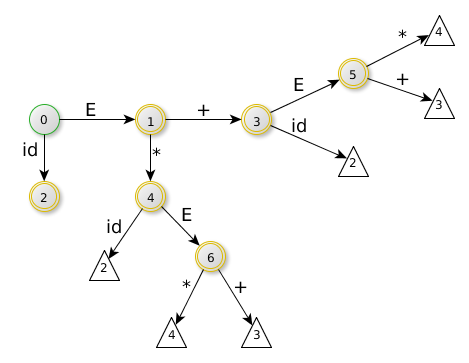
\includegraphics[scale=0.4]{Chapters/Img/c02_17.png}\\
\end{center} 

//Se va a triangoli, non parte dal kernel, altrimenti si(?)

0 =
\begin{tabular}{l}
	$E' \rightarrow .E$		\\
	$E \rightarrow .E + E$	\\
	$E \rightarrow .E * E$	\\
	$E \rightarrow .id$		\\
\end{tabular}

1 =
\begin{tabular}{l}
	$E' \rightarrow E.$		\\
	$E \rightarrow E. + E$	\\
	$E \rightarrow E. * E$	\\
\end{tabular}

2 =
\begin{tabular}{l}
	$E \rightarrow id.$		\\
\end{tabular}

3 =
\begin{tabular}{l}
	$E \rightarrow E + .E$		\\
	$E \rightarrow .E * E$		\\
	$E \rightarrow .id $		\\
\end{tabular}

4 =
\begin{tabular}{l}
	$E \rightarrow E * .E$		\\
	$E \rightarrow .E + E$		\\
	$E \rightarrow .E * E$		\\
	$E \rightarrow .id $		\\
\end{tabular}

5 =
\begin{tabular}{l}
	$E \rightarrow E + E.$		\\
	$E \rightarrow E. + E$		\\
	$E \rightarrow E. * E$		\\
\end{tabular}

6 =
\begin{tabular}{l}
	$E \rightarrow E * E.$		\\
	$E \rightarrow E. + E$		\\
	$E \rightarrow E. * E$		\\
\end{tabular}

\begin{tabular}{|c|c|c|c|c|}
		&	id 		&	+	&	*	&	$ \$ $	\\
	0	&	S2 		&		&		&			\\	
	1	&	 		&	S3	&	S4	&	ACCEPT	\\	
	2	&	 		&	$R:\ E \rightarrow id $		&	$R:\ E \rightarrow id $	& $R:\ E \rightarrow id $	\\	
	3	&	S2 		&		&		&			\\	
	4	&	S2 		&		&		&			\\	
	5	&	 		&	$S3,\ R:\ E \rightarrow E+E$	&	$S4,\ R:\ E \rightarrow E+E$	&	$R:\ E \rightarrow E+E$		\\	
	6	&	S2 		&	$S3,\ R:\ E \rightarrow E*E$	&	$S4,\ R:\ E \rightarrow E*E$	&	$R:\ E \rightarrow E*E$		\\	
\end{tabular}

Visto che ci sono conflitti nella tabella, questa grammatica non \'e SLR. In questo caso i conflitti sono di tipo Shift/Reduce.
Ma possono essere anche di tipo Reduce/Reduce.

Tra le produzioni nelle celle colorate, quali sono quelle da tenere per avere una grammatica che associa a sinistra?

Nella cella [5, +] devo tenere R \lq\lq $E \rightarrow E + E $ \rq\rq\\
Nella cella [5, *] devo tenereS4 \\
Nella cella [6, +] devo tenere R \lq\lq $E \rightarrow E * E $ \rq\rq\\
Nella cella [6, *] devo tenere R \lq\lq $E \rightarrow E * E $ \rq\rq\\  

$W = id * id + id \$ $\\
$ 0 $\\
$ 0id2 $\\
$ 0E1 $\\
$ 0E1*4id2 $\\
$ 0E1*4E6 $\\
$ 0E1 $\\
$ 0E1+3id2 $\\
$ 0E1+3E5 $\\
$ 0E1 $\\
$ ok $\\

\Tree[.E [.E [.E id] * [.E id ] ] + [.E id ] ]

\subsection{Esempio}
$S \rightarrow aAd | bBd | aBe | bAe$\\
$A \rightarrow c $\\
$B \rightarrow c $\\

Questa grammatica produce 4 stringhe, ogniuna in un modo, e quindi ovviamente non \'e ambigua.

\begin{center}
    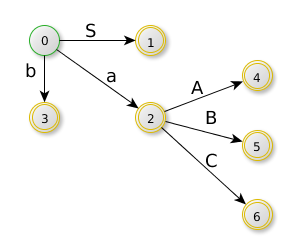
\includegraphics[scale=0.4]{Chapters/Img/c02_18.png}\\
\end{center} 

0 =
\begin{tabular}{l}
	$S' \rightarrow .S $		\\
	$S  \rightarrow .aAd $		\\
	$S  \rightarrow .bBd $		\\
	$S  \rightarrow .aBe $		\\
	$S  \rightarrow .bAe $		\\
\end{tabular}

1 =
\begin{tabular}{l}
	$S' \rightarrow S. $		\\
\end{tabular}

2 =
\begin{tabular}{l}
	$S \rightarrow a.Ad  $		\\
	$S  \rightarrow a.Be $		\\
	$A  \rightarrow .c $		\\
	$B  \rightarrow .c $		\\
\end{tabular}

3 =
\begin{tabular}{l}
	$S \rightarrow b.Bd  $		\\
	$S  \rightarrow b.Ae $		\\
	$B  \rightarrow .c $		\\
	$A  \rightarrow .c $		\\
\end{tabular}

4 =
\begin{tabular}{l}
	$S \rightarrow aA.d $		\\
\end{tabular}

5 =
\begin{tabular}{l}
	$S \rightarrow aB.e $		\\
\end{tabular}

6 =
\begin{tabular}{l}
	$A \rightarrow c. $		\\
	$B \rightarrow c. $		\\
\end{tabular}

\begin{tabular}{|c|c|c|c|c|c|}
	\hline
		&	a 	& 	b 	&	d 	& 	e 	&	$\$$ 	\\
	\hline
	6	&	 	& 	$R:\ A \rightarrow c $ 	&	$R:\ A \rightarrow c $ 	& 	& 	\\	
		&	 	& 	$R:\ B \rightarrow c $ 	&	$R:\ B \rightarrow c $ 	& 	& 	\\	
	\hline
\end{tabular}

Anche se non \'e una grammatica ambigua ci sono multiple entries. Questo dipende dal modo in cui scegliamo i follow. 
Nel parsing canonico infatti non si usano gli item LR(0) ma gli item LR(1) perch\'e ci postiamo dietro informazione direttamente
dagli item. Questo riduce/rimuove i problemi di questo tipo.

Un item LR(1) canonico \'e del tipo $A \rightarrow \alpha . \beta, \delta$ con $\delta \subset T \cup \{ \$ \}$.\\

\section{LR(1)}
Negli automi caratteristici LR(1) si considera come stato iniziale lo stato che si ottiene facendo: 
$closure_1 (\{[ S' \rightarrow .S, \{ \$\}  ]\})$

\subsection{Esempio}
